% !TEX root= ../main.tex
\section{Inconsistencies in graph theories}
\label{sec:Inconsistencies in graph theories}
In this section, we will prove the existence of non-binary-derivable inconsistencies from graphs.
We will first prove a lemma, then apply this lemma to an extended version of the graph from Figure~\ref{fig:double_open_door} to show that its inconsistency is not binary-derivable.

Let $\mathbf{G} = \langle G,N \rangle$ be a digraph with a source vertex $x$.
Let $\{A_i\}$ be a \textit{partitioning} of $G \setminus \{ x \}$ (a set of pairwise disjoint, nonempty subsets of $G$ such that $\bigcup \{A_i\} = G \setminus \{ x \}$) such that for each $A_i$ we have that $N(A_i) \subseteq A_i$ and $N^-(A_i) \setminus A_i = \{ x \}$.
In words, nothing points out of $A_i$ and only $x$ points in.

The induced subgraphs we get from each $A_i$ will be referred to as \textit{components}.\par
\begin{figure}[!h]
  \centering
  \begin{tikzpicture}
    [
    point/.style={circle,draw,inner sep=0pt,minimum size=2mm},
    collection/.style={rectangle,draw,inner sep=0pt,minimum height=10mm, minimum width= 18mm}
    ]
    \node (x) at (3,2) [point, label=above:$x$] {};
    \node (A1) at (0,0) [collection] {$A_1$};
    \node (A2) at (2,0) [collection] {$A_2$};
    \node (dots) at (4,0) [] {\dots};
    \node (An) at (6,0) [collection] {$A_n$};
    \draw [-latex] (x) to (A1);
    \draw [-latex] (x) to (A2);
    \draw [-latex, dashed] (x) to (dots);
    \draw [-latex] (x) to (An);
  \end{tikzpicture}
  \caption{Graph $G$}
  \label{fig:components_link}
\end{figure}
A couple of observations can be made based on the above graph-construction $G$:
\begin{itemize}
  \item The vertex $x$ only appears in 1 OR-clause, since it is a source vertex.
  This is also the only OR-clause containing vertices from different components.
  We will call this OR-clause $X$ and formally define it as $N(x) \cup \{ x\}$.
  \item For any vertex $p$ except $x$, we have that $p$ only appears in axiomatic NAND-clauses together with either $x$ or other vertices in the same component.
\end{itemize}
Based on graph $G$ from Figure~\ref{fig:components_link} we show the following lemma:
\begin{lemma}
  For arbitrary vertices $a_i \in A_i$ and $a_j \in A_j$ such that $i \neq j$; if $\ol{a_ia_j}$ is provable in BNeg, then the proof must contain the OR-clause $X$.
  \label{thm:or_clause_lemma}
\end{lemma}
\begin{proof}
  The lemma will be proven by structural induction on the complexity of the proof tree for $\ol{a_ia_j}$.

  In the base case, the proof tree is just an axiom.
  $\ol{a_ia_j}$ is not an axiom, since $\bigcap_i N(A_i) = \varnothing$, so the lemma holds vacuously.

  For the inductive step, suppose we have a proof of $\ol{a_ia_j}$ and consider the premise of the last rule application;
  since we are working within BNeg, this premise must contain one NAND-clause on the form $\ol{a_ip}$ and one on the form $\ol{a_iq}$.
  The following figure illustrates the situation:\par
  \begin{figure}[!h]
    \centering
    \begin{prooftree*}
      \Hypo{\dots}
      \Infer[]1{\ol{a_ip}}
      \Hypo{\dots}
      \Infer[]1{\ol{a_jq}}
      \Hypo{\dots}
      \Infer[right label=$Y$]3{\ol{a_ia_j}}
    \end{prooftree*}
    \caption{}
    \label{fig:ab_proof_bc}
  \end{figure}
  \FloatBarrier
  First, with either $p = x$ or $q = x$, the OR-clause $Y$ used in the proof step must be $X$, being the only OR-clause containing $x$.
  This case gives the claim.
  Otherwise, our induction hypothesis gives us that any NAND-clause $\ol{cd}$ in the premise, such that $c$ and $d$ are from different components, must have a proof containing the OR-clause $X$.
  Therefore, in order to avoid $X$ earlier in the proof, $p$ and $q$ must come from $A_i$ and $A_j$, respectively.
  Since $X$ is the only OR-clause containing vertices from both $A_i$ and $A_j$, $X$ is again our only option.
  The proof of $\ol{a_ia_j}$ must therefore contain the OR-clause $X$.
\end{proof}
\begin{figure}[!h]
  \centering
  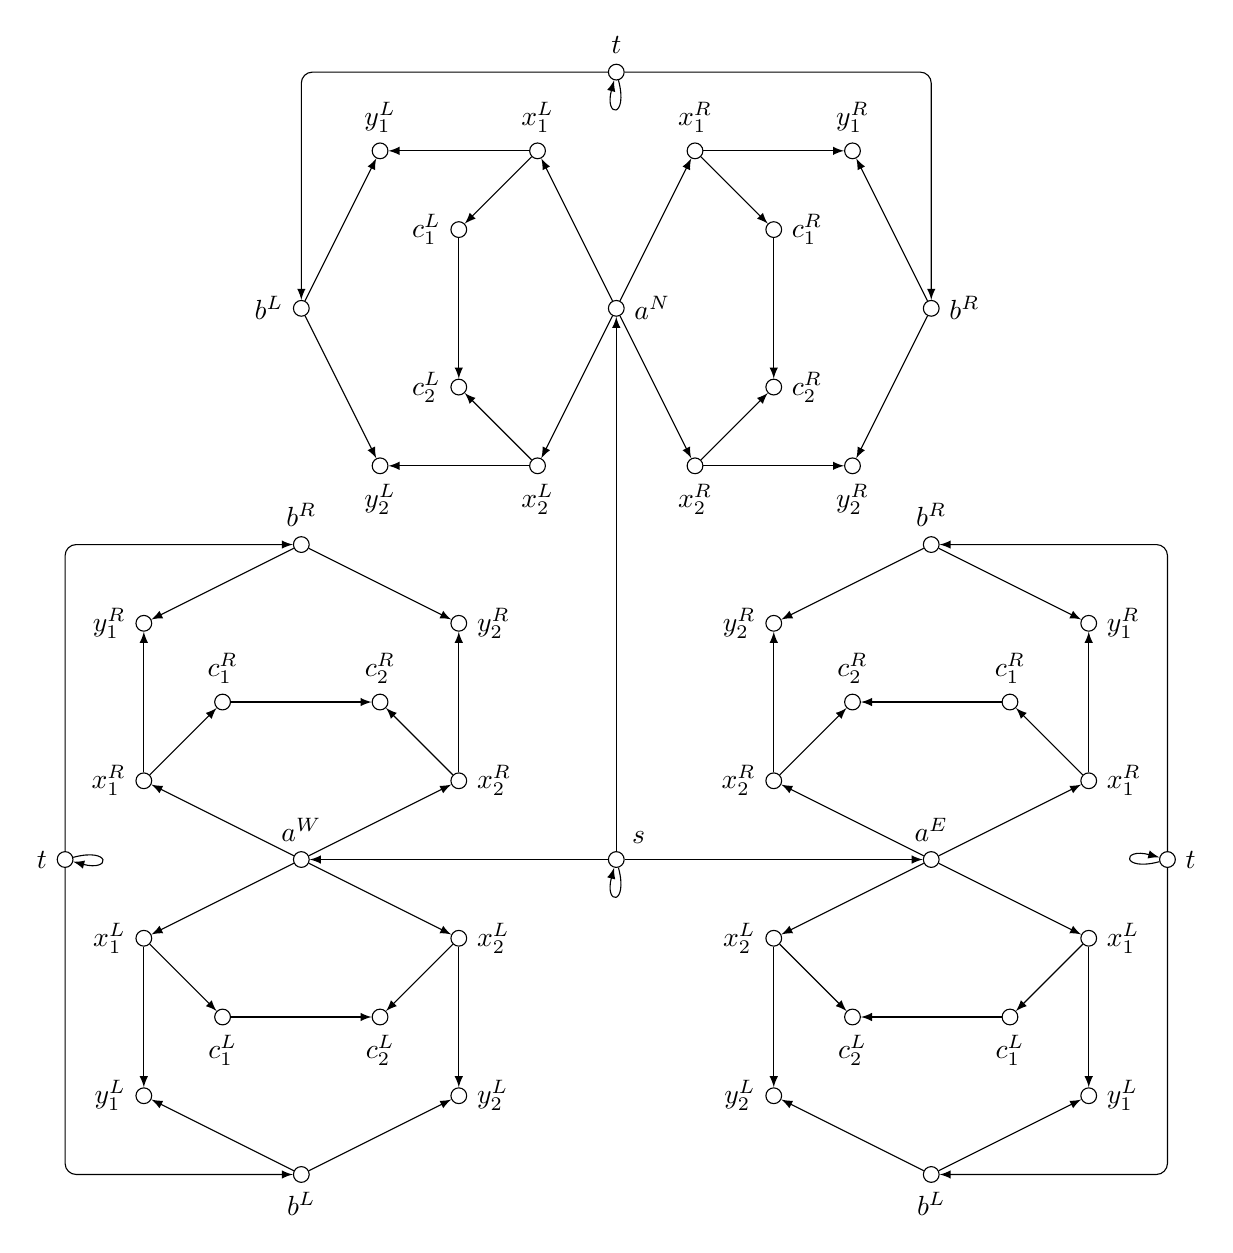
\begin{tikzpicture}
    [
    point/.style={circle,draw,inner sep=0pt,minimum size=2mm}
    ]
    \node (t) at (7,14) [point,label=above:$t$] {};
    \node (a) at (7,11) [point,label=right:$a^N$] {};
    \node (lx1) at (6,13) [point,label=above:$x^L_1$] {};
    \node (lx2) at (6,9) [point,label=below:$x^L_2$] {};
    \node (lb) at (3,11) [point,label=left:$b^L$] {};
    \node (ly1) at (4,13) [point,label=above:$y^L_1$] {};
    \node (ly2) at (4,9) [point,label=below:$y^L_2$] {};
    \node (lc1) at (5,12) [point,label=left:$c^L_1$] {};
    \node (lc2) at (5,10) [point,label=left:$c^L_2$] {};
    \draw [-latex] (a) to (lx1);
    \draw [-latex] (a) to (lx2);
    \draw [-latex] (lb) to (ly1);
    \draw [-latex] (lb) to (ly2);
    \draw [-latex] (lx1) to (ly1);
    \draw [-latex] (lx1) to (lc1);
    \draw [-latex] (lx2) to (ly2);
    \draw [-latex] (lx2) to (lc2);
    \draw [-latex] (lc1) to (lc2);
    \node (rx1) at (8,13) [point,label=above:$x^R_1$] {};
    \node (rx2) at (8,9) [point,label=below:$x^R_2$] {};
    \node (rb) at (11,11) [point,label=right:$b^R$] {};
    \node (ry1) at (10,13) [point,label=above:$y^R_1$] {};
    \node (ry2) at (10,9) [point,label=below:$y^R_2$] {};
    \node (rc1) at (9,12) [point,label=right:$c^R_1$] {};
    \node (rc2) at (9,10) [point,label=right:$c^R_2$] {};
    \draw [-latex] (a) to (rx1);
    \draw [-latex] (a) to (rx2);
    \draw [-latex] (rb) to (ry1);
    \draw [-latex] (rb) to (ry2);
    \draw [-latex] (rx1) to (ry1);
    \draw [-latex] (rx1) to (rc1);
    \draw [-latex] (rx2) to (ry2);
    \draw [-latex] (rx2) to (rc2);
    \draw [-latex] (rc1) to (rc2);
    \draw [-latex, rounded corners] (t) -| (lb);
    \draw [-latex, rounded corners] (t) -| (rb);
    \draw [-latex, loop below] (t) to (t);

    \node (wt) at (0,4) [point,label=left:$t$] {};
    \node (wa) at (3,4) [point,label=above:$a^W$] {};
    \node (wlx1) at (1,3) [point,label=left:$x^L_1$] {};
    \node (wlx2) at (5,3) [point,label=right:$x^L_2$] {};
    \node (wlb) at (3,0) [point,label=below:$b^L$] {};
    \node (wly1) at (1,1) [point,label=left:$y^L_1$] {};
    \node (wly2) at (5,1) [point,label=right:$y^L_2$] {};
    \node (wlc1) at (2,2) [point,label=below:$c^L_1$] {};
    \node (wlc2) at (4,2) [point,label=below:$c^L_2$] {};
    \draw [-latex] (wa) to (wlx1);
    \draw [-latex] (wa) to (wlx2);
    \draw [-latex] (wlb) to (wly1);
    \draw [-latex] (wlb) to (wly2);
    \draw [-latex] (wlx1) to (wly1);
    \draw [-latex] (wlx1) to (wlc1);
    \draw [-latex] (wlx2) to (wly2);
    \draw [-latex] (wlx2) to (wlc2);
    \draw [-latex] (wlc1) to (wlc2);
    \node (wrx1) at (1,5) [point,label=left:$x^R_1$] {};
    \node (wrx2) at (5,5) [point,label=right:$x^R_2$] {};
    \node (wrb) at (3,8) [point,label=above:$b^R$] {};
    \node (wry1) at (1,7) [point,label=left:$y^R_1$] {};
    \node (wry2) at (5,7) [point,label=right:$y^R_2$] {};
    \node (wrc1) at (2,6) [point,label=above:$c^R_1$] {};
    \node (wrc2) at (4,6) [point,label=above:$c^R_2$] {};
    \draw [-latex] (wa) to (wrx1);
    \draw [-latex] (wa) to (wrx2);
    \draw [-latex] (wrb) to (wry1);
    \draw [-latex] (wrb) to (wry2);
    \draw [-latex] (wrx1) to (wry1);
    \draw [-latex] (wrx1) to (wrc1);
    \draw [-latex] (wrx2) to (wry2);
    \draw [-latex] (wrx2) to (wrc2);
    \draw [-latex] (wrc1) to (wrc2);
    \draw [-latex, rounded corners] (wt) |- (wlb);
    \draw [-latex, rounded corners] (wt) |- (wrb);
    \draw [-latex, loop right] (wt) to (wt);

    \node (et) at (14,4) [point,label=right:$t$] {};
    \node (ea) at (11,4) [point,label=above:$a^E$] {};
    \node (elx1) at (13,3) [point,label=right:$x^L_1$] {};
    \node (elx2) at (9,3) [point,label=left:$x^L_2$] {};
    \node (elb) at (11,0) [point,label=below:$b^L$] {};
    \node (ely1) at (13,1) [point,label=right:$y^L_1$] {};
    \node (ely2) at (9,1) [point,label=left:$y^L_2$] {};
    \node (elc1) at (12,2) [point,label=below:$c^L_1$] {};
    \node (elc2) at (10,2) [point,label=below:$c^L_2$] {};
    \draw [-latex] (ea) to (elx1);
    \draw [-latex] (ea) to (elx2);
    \draw [-latex] (elb) to (ely1);
    \draw [-latex] (elb) to (ely2);
    \draw [-latex] (elx1) to (ely1);
    \draw [-latex] (elx1) to (elc1);
    \draw [-latex] (elx2) to (ely2);
    \draw [-latex] (elx2) to (elc2);
    \draw [-latex] (elc1) to (elc2);
    \node (erx1) at (13,5) [point,label=right:$x^R_1$] {};
    \node (erx2) at (9,5) [point,label=left:$x^R_2$] {};
    \node (erb) at (11,8) [point,label=above:$b^R$] {};
    \node (ery1) at (13,7) [point,label=right:$y^R_1$] {};
    \node (ery2) at (9,7) [point,label=left:$y^R_2$] {};
    \node (erc1) at (12,6) [point,label=above:$c^R_1$] {};
    \node (erc2) at (10,6) [point,label=above:$c^R_2$] {};
    \draw [-latex] (ea) to (erx1);
    \draw [-latex] (ea) to (erx2);
    \draw [-latex] (erb) to (ery1);
    \draw [-latex] (erb) to (ery2);
    \draw [-latex] (erx1) to (ery1);
    \draw [-latex] (erx1) to (erc1);
    \draw [-latex] (erx2) to (ery2);
    \draw [-latex] (erx2) to (erc2);
    \draw [-latex] (erc1) to (erc2);
    \draw [-latex, rounded corners] (et) |- (elb);
    \draw [-latex, rounded corners] (et) |- (erb);
    \draw [-latex, loop left] (et) to (et);

    \node (s) at (7,4) [point,label=above right:$s$] {};
    \draw [-latex] (s) to (a);
    \draw [-latex] (s) to (wa);
    \draw [-latex] (s) to (ea);
    \draw [-latex,loop below] (s) to (s);
  \end{tikzpicture}
  \caption{}
  \label{fig:triple_double_open_door}
\end{figure}
\FloatBarrier
Consider now the graph in Figure~\ref{fig:triple_double_open_door} containing 3 copies of our graph from Figure~\ref{fig:double_open_door}; one northern (N), one western (W) and one eastern (E).
We will refer to these as components.

The proof of $\ol{a}$ from Figure~\ref{fig:unary_nand_proof} can be applied to each component in the above graph, giving us the provability of $\ol{a^N}$, $\ol{a^W}$ and $\ol{a^E}$.
From here, the inconsistency proof is trivial; shown in Figure~\ref{fig:triple_double_open_door_proof}.\par
\begin{figure}[!h]
  \centering
  \begin{prooftree*}
    \Hypo{\ol{s}}
    \Hypo{\dots}
    \Infer[]1{\ol{a^N}}
    \Hypo{\dots}
    \Infer[]1{\ol{a^W}}
    \Hypo{\dots}
    \Infer[]1{\ol{a^E}}
    \Infer[right label=$sa^Na^Wa^E$]4{\varnothing}
  \end{prooftree*}
  \caption{}
  \label{fig:triple_double_open_door_proof}
\end{figure}
The graph is thus provably inconsistent.

We will now use Lemma~\ref{thm:or_clause_lemma} to prove the following lemma:
\begin{lemma}
  Given any of the three $a$-vertices in the graph in Figure~\ref{fig:triple_double_open_door}, if $\ol{a}$ is binary-derivable, then its proof contains the OR-clause $sa^Na^Wa^E$.
  \label{thm:a_binary_derivable}
\end{lemma}
\begin{proof}
  Suppose, without any loss of generality, that $a^N$ is the vertex such that $\ol{a^N}$ is binary-derivable.
  From Section~\ref{sec:Unary NAND-clauses in graph theories} we get that $\ol{a^N}$ is not binary-derivable using clauses from the N-component only.
  Therefore, its proof must contain NAND-clauses containing either the vertex $s$ or some vertex from the two other components.

  If its proof contains some NAND-clause containing $s$, then the proof must also have a step removing this $s$, since we do not want that atom in our conclusion.
  The OR-clause $sa^Na^Wa^E$ is the only clause that can do this, being the only OR-clause containing $s$.

  If its proof contains NAND-clauses with vertices from component W or E (let us call them \textit{external clauses}), then consider the proof step where they last appear.
  Either all external clauses appear as unary NAND-clauses or at least one of them appear as a binary NAND-clause.
  If one external clause is binary then it cannot contain two vertices from outside component $N$, because only one of the two vertices would be removed in that step, so it would not possibly be the last appearance of an external clause.
  Therefore, the binary clause must contain one vertex from the N-component and one from outside.
  Lemma~\ref{thm:or_clause_lemma} gives us that $sa^Na^Wa^E$ must have been used to prove it.

  If all the external clauses are unary, in order to not prove $\varnothing$, one clause must be binary and from the N-component.
  Since $sa^Na^Wa^E$ is the only OR-clause containing vertices from different components, this is the OR-clause that must be used.
\end{proof}

We will now show that the inconsistency of the graph in Figure~\ref{fig:triple_double_open_door} is non-binary-derivable.
\begin{proof}
The first thing to notice is that if one removes the loop on vertex $s$, the graph is no longer inconsistent.
This tells us that the NAND-clause $\ol{s}$ must be a part of every inconsistency proof.
If that was not the case, we would be able to prove $\varnothing$ on a consistent graph, violating the fact that Neg is sound.

Having that any inconsistency proof contains $\ol{s}$ immediately gives us that any inconsistency proof contains the OR-clause $sa^Na^Wa^E$, since this is the only OR-clause containing $s$.
The OR-clause in question might obviously appear several places in the proof, so let us assume that the proof step in Figure~\ref{fig:triple_double_proof_step} is its \textit{first} appearance i.e. none of the NAND-clauses in the premise are proven using the OR-clause $sa^Na^Wa^E$.
Note that this first appearance might not have the axiom $\ol{s}$ in its premise, but rather some other NAND-clause containing $s$.\par
\begin{figure}[!h]
  \centering
  \begin{prooftree*}
    \Hypo{\dots}
    \Infer[]1{\ol{sM}}
    \Hypo{\dots}
    \Infer[]1{\ol{a^NP}}
    \Hypo{\dots}
    \Infer[]1{\ol{a^WQ}}
    \Hypo{\dots}
    \Infer[]1{\ol{a^WR}}
    \Infer[right label=$sa^Na^Wa^E$]4{\ol{M \cup P \cup Q \cup R}}
  \end{prooftree*}
  \caption{First appearance of $sa^Na^Wa^E$. $M,P,Q,R$ being possibly empty}
  \label{fig:triple_double_proof_step}
\end{figure}
First of all, neither of the sets $M,P,Q,R$ can contain more than 1 element, since that would make the NAND-clause containing them non-binary.
For the same reason can their union never contain more than two elements, since that would make the concluding NAND-clause non-binary.
Therefore, either two of the four sets are empty, or some of them contain the same element.

Let us first look at the case where two of them are empty.
The unary NAND-clause $\ol{s}$ is an axiom, so $M$ being empty is not problematic.
We have however just showed in Lemma~\ref{thm:a_binary_derivable} that if any of the unary NAND-clauses $\ol{a^N}$, $\ol{a^W}$ or $\ol{a^E}$ are binary-derivable, then their proof must contain $sa^Na^Wa^E$, contradicting our original assumption of it being used for the first time in Figure~\ref{fig:triple_double_proof_step}.

This leaves us with the second option where $P,Q,R$ are all nonempty.
In order for the concluding NAND-clause to be binary, two of the three sets $P,Q,R$ must contain the same element.
We will apply Lemma~\ref{thm:or_clause_lemma} to show that this is not possible.

Let, without any loss of generality, $P$ and $Q$ be the two sets containing the same element, i.e. $P = Q = \{p\}$, giving us the two NAND-clauses $\ol{a^Np}$ and $\ol{a^Wp}$.
If $p \neq s$, we get the situation where $p$ must be in a component different from either $a^N$ or $a^W$, since $a^N$ and $a^W$ are in different components.
From this, Lemma~\ref{thm:or_clause_lemma} gives us that the proof of that NAND-clause must contain the OR-clause $sa^Na^Wa^E$, which contradicts our assumption of it being used for the first time in Figure~\ref{fig:triple_double_proof_step}.

The only option left at this point is the one where $p = s$, i.e. the case where $\ol{a^Ns}$ and $\ol{a^Ws}$ appear in the premise.
In this case, the conclusion will always contain $s$ leaving us with no OR-clauses are able to remove $s$-vertices from clauses in the premise.
Since $s$ must be a part of the proof, and we have no way of removing it, reaching $\varnothing$ is impossible.

The inconsistency in Figure~\ref{fig:triple_double_open_door} is thus not binary-derivable.
\end{proof}
